\documentclass{beamer}

% Setup appearance:

\usetheme{Darmstadt}
\usecolortheme{albatross}
\usefonttheme[onlylarge]{structurebold}
\setbeamerfont*{frametitle}{size=\normalsize,series=\bfseries}
\setbeamertemplate{navigation symbols}{}

% Redefine the colors to make them closer to mmm.
\definecolor{MWBlood}{rgb}{0.278, 0.0, 0.016} % MWBlood (primary)
\definecolor{MWBloodDark}{rgb}{0.039, 0.0, 0.0} % MWBloodDark (secondary)
\definecolor{MWBloodMiddle}{rgb}{0.171, 0.00, 0.01} % MWBloodMiddle ()
\definecolor{MWBone}{rgb}{0.827, 0.827, 0.827} % MWBone (Text)

\setbeamercolor*{normal text}{fg=MWBone!50!white,bg=MWBloodMiddle!50!MWBlood} % TOC subsection and more important the dropshadow.
\setbeamercolor*{structure}{fg=MWBlood!25!MWBone} % Section heading color in TOC and inside of enum circles.

\setbeamercolor{palette primary}{bg=MWBlood,fg=MWBone} % Slide heading and title box background.
\setbeamercolor{palette secondary}{bg=MWBloodMiddle, fg=MWBone}
\setbeamercolor{palette tertiary}{bg=green,fg=MWBone}
\setbeamercolor{palette quaternary}{bg=MWBloodDark, fg=MWBone} % Navigation bar
\setbeamercolor{background canvas}{bg=MWBloodDark, fg=green} % Slide background

% Standard packages

\usepackage{times}
\usepackage[utf8]{inputenc}
\usepackage[greek,english]{babel}

\usepackage{url}
\usepackage{lettrine}
\usepackage{hyperref}

\usepackage{listings}

% Setup TikZ

\usepackage{tikz}
\usetikzlibrary{arrows}
\tikzstyle{block}=[draw opacity=0.7,line width=1.4cm]

% Author, Title, etc.

\title[Titel]
{
  \texttt{\huge{meta metal mapper}}\\\vspace{3 mm}
  \textit{A data science and Python journey for software developers}
}

\author[Martin Woelke]
{
  Martin~Woelke
}

\date{Lübeck - \today}

% The main document

\begin{document}

\begin{frame}
  \titlepage
\end{frame}


\section{Introduction}

%\pgfimage[width=.45\textwidth,page=2]{beamer}

  \subsection{Overview}

    \begin{frame}{Summary}
      \tableofcontents
    \end{frame}

  \subsection{The Music}

    \begin{frame}{What does the quirky name mean?}
      \begin{itemize}
        \item\textbf{Meta} (from the Greek meta- \foreignlanguage{greek}{μετά}- meaning
        "after" or "beyond") is a prefix meaning more comprehensive or transcending\footnotemark.\pause
        \item\textbf{Metal}: A style of contemporary rock  music.\pause
        \item\textbf{Mapper}: An entity making a symbolic depiction emphasizing relationships
        between elements of some space, such as objects, regions, or themes.\pause
      \end{itemize}
      
      \vspace{5mm}
      
      And there are already commercial products searching for metal (in the ground).
      
      \footnotetext[1]{https://en.wikipedia.org/wiki/Meta}
      
    \end{frame}

    \begin{frame}{Origins of metal}
      \begin{center}
        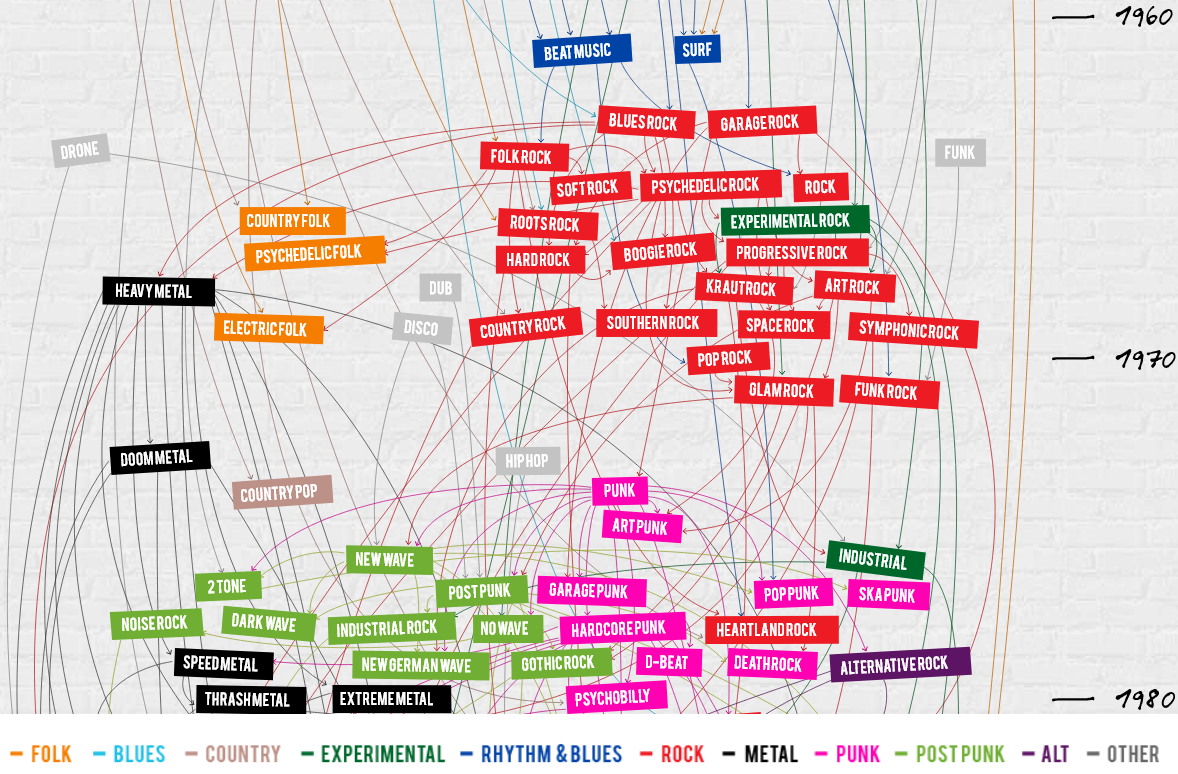
\includegraphics[scale=.33]{familyTree2}
      \end{center}
      \href{https://www.concerthotels.com/100-years-of-rock/}{https://www.concerthotels.com/100-years-of-rock/}
    \end{frame}

    \begin{frame}{What is metal?}
%      \uncover<1-1>
      \pause
      \begin{center}
        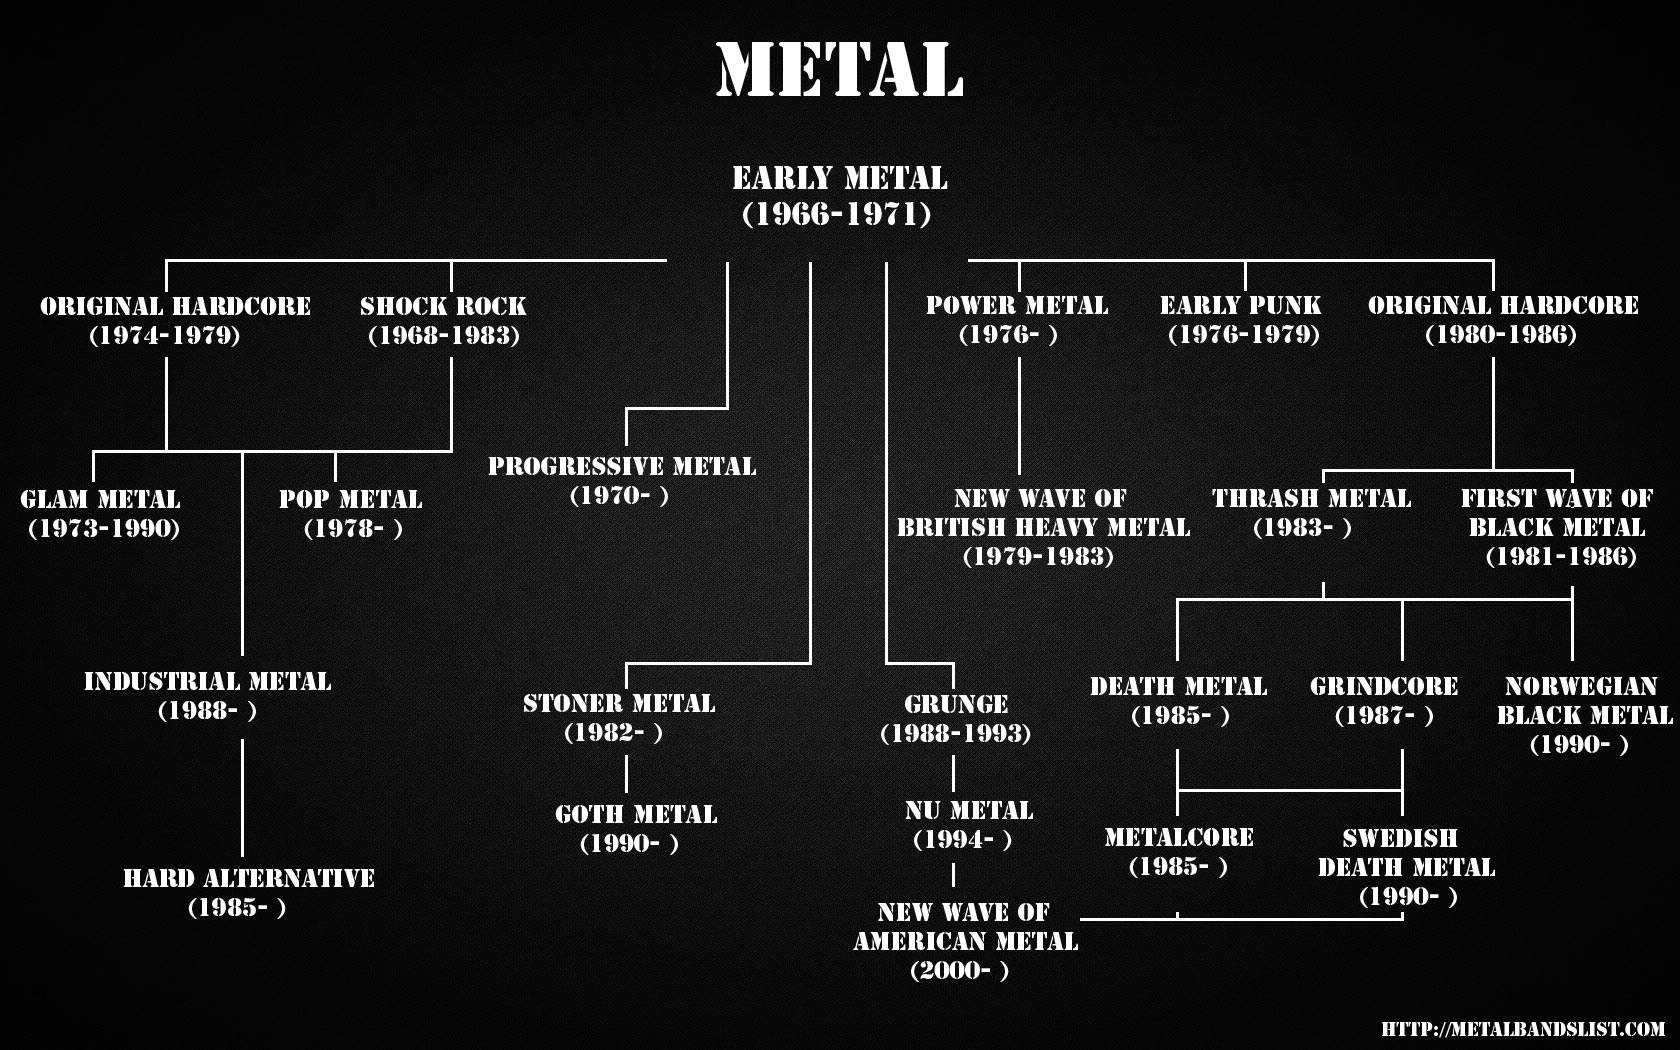
\includegraphics[scale=.18]{familyTree}
      \end{center}
    \end{frame}

    \begin{frame}{What is metal?}

      \begin{block}{Wikipedia Definition}
        Heavy metal (or simply metal) is a genre of rock music that developed in the late 1960s
        and early 1970s, largely in the United Kingdom. With roots in blues rock, psychedelic
        rock, acid rock, the bands that created heavy metal developed a thick, massive sound,
        characterized by highly amplified distortion, extended guitar solos, emphatic beats,
        and overall loudness.\footnote{https://en.wikipedia.org/wiki/Heavy\_metal\_music}
      \end{block}

    \end{frame}

  \subsection{meta metal mapper}

    \begin{frame}{Inspiration}
    
      From the liner notes of \textit{True Kings of Norway}:
    
      \begin{center}
        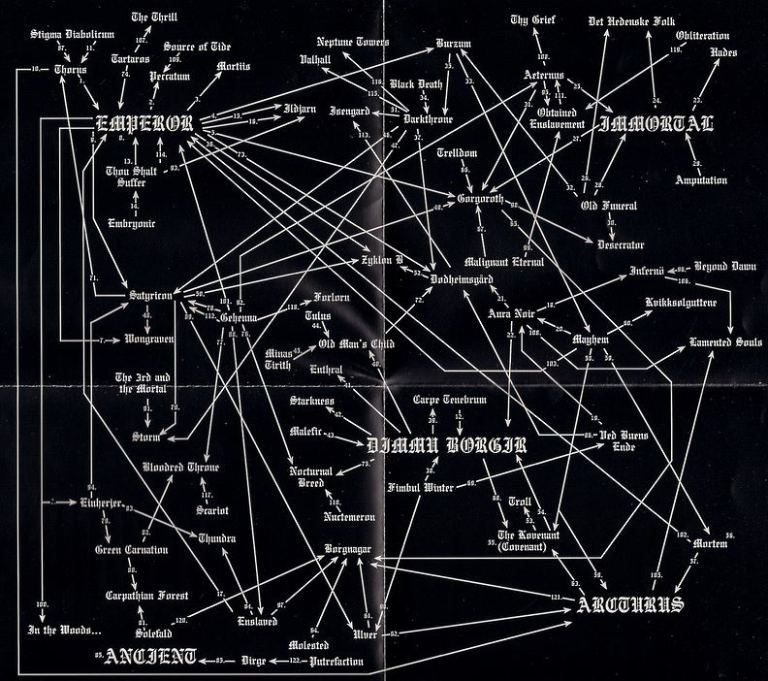
\includegraphics[scale=2.3]{true_kings_diagram}
      \end{center}
      
    \end{frame}
    
    \begin{frame}{Encyclopaedia Metallum: The Metal Archives}
    
      \begin{itemize}
        \item \textit{The} website for anything metal.
        \item Started in 2002.
        \item 134346 bands from 151 countries (March 2020).
      \end{itemize}
    
      \begin{center}
        
\includegraphics[scale=.4]{MA_banner}
      \end{center}
      
      https://www.metal-archives.com/
      
    \end{frame}

\section{Development}

  \subsection{Humble beginnings}

    \begin{frame}{What the..... data!}
    
      \begin{center}
        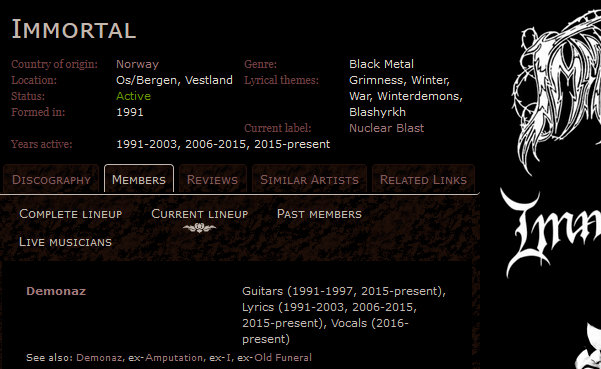
\includegraphics[scale=2]{MA_Immortal}
      \end{center}
    
    \end{frame}

    \begin{frame}{History}

      \begin{itemize}

        \item<1-> First commit: 2014-03-15
        \item<1-> Some progress made till July.
          \begin{center}
            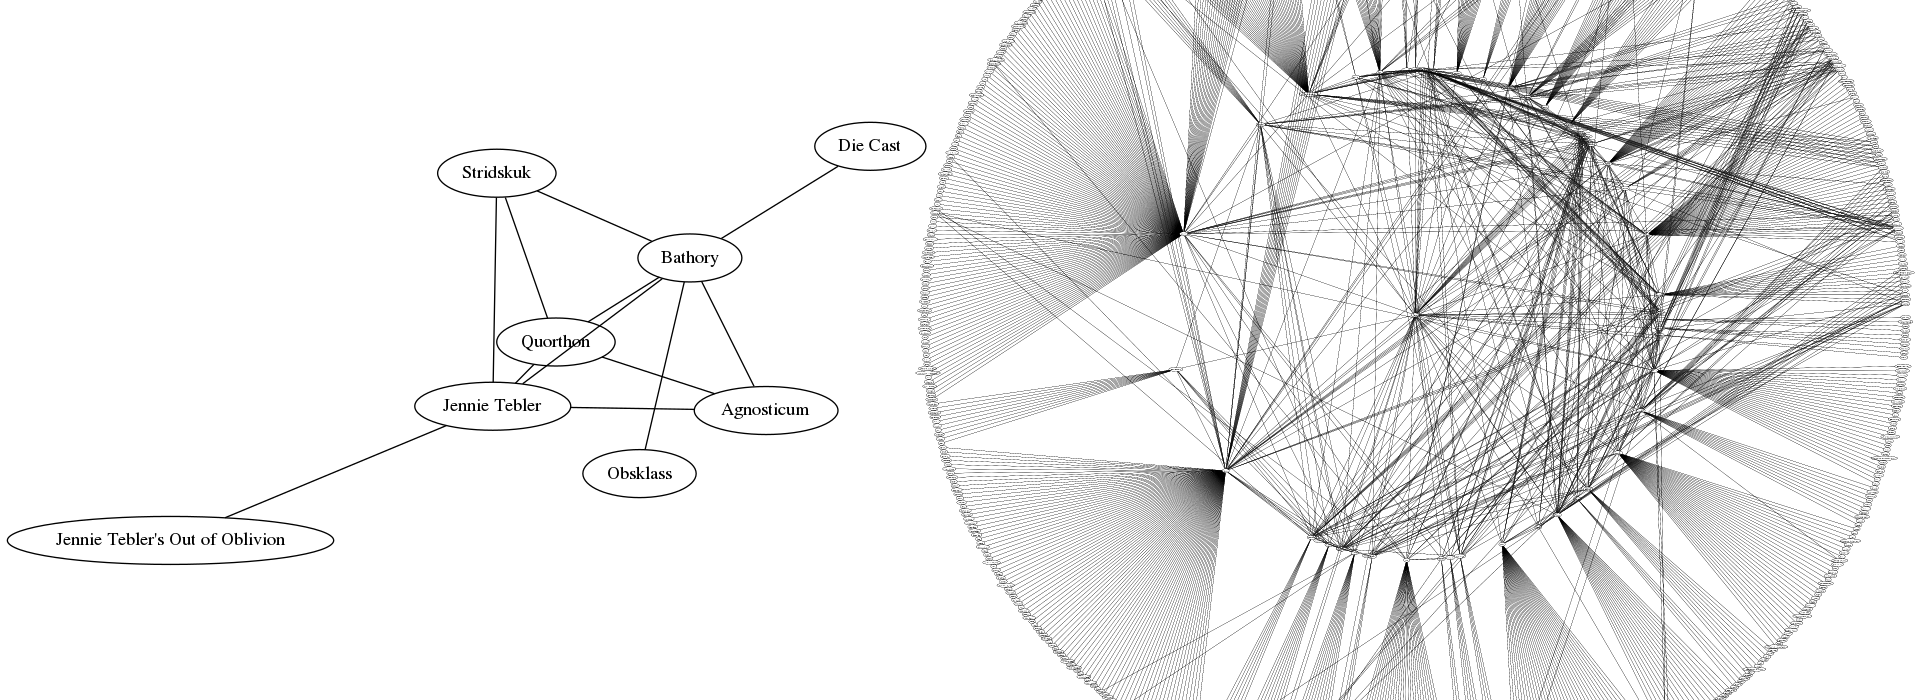
\includegraphics[scale=.6]{bandsGraphCombined}
          \end{center}
        \item<2-> Mothballed until end of 2018.
        \item<2-> Found graph databases while reading about connected data
          (a.k.a. networks).
        \item<2-> Converted codebase to Python3 and started using a debugger.
      \end{itemize}

    \end{frame}
    
  \subsection{Getting data from webpages with BeautifulSoup}
  
    \begin{frame}{Web Page Reverse Engineering}
    
      Firefox' onboard web deloper tools.
    
      \begin{center}
        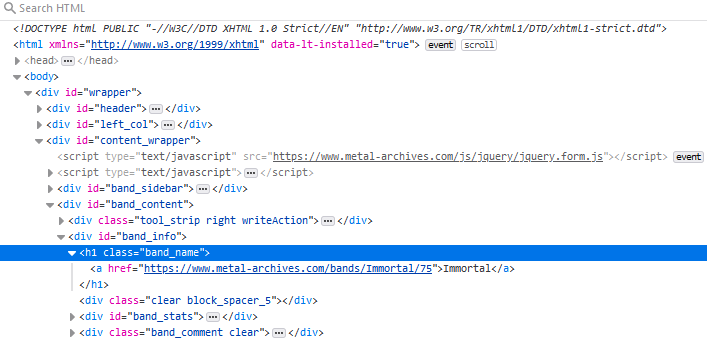
\includegraphics[scale=.6]{firefox_dom}
      \end{center}
    
    \end{frame}   
    
    %\begin{frame}{Getting a page and parse data}[fragile]
    \begin{frame}[fragile]

How to get any data from any webpage:

\begin{lstlisting}[basicstyle=\footnotesize,]

link = "https://www.metal-archives.com/bands/Immortal/75"
http = urllib3.PoolManager(
  cert_reqs='CERT_REQUIRED' , ca_certs=certifi.where())
web_page = http.request('GET', link)
web_page_string = web_page.data.decode("utf-8")
soup = BeautifulSoup(web_page.data.decode(
  'utf-8', 'ignore'), "html.parser")
s = band_soup.find_all(attrs={"class": "band_name"})

\end{lstlisting}

    \end{frame}

    \begin{frame}{Example: BeautifulSoup}

      Debugging the found \texttt{ResultSet}:

      \begin{center}
        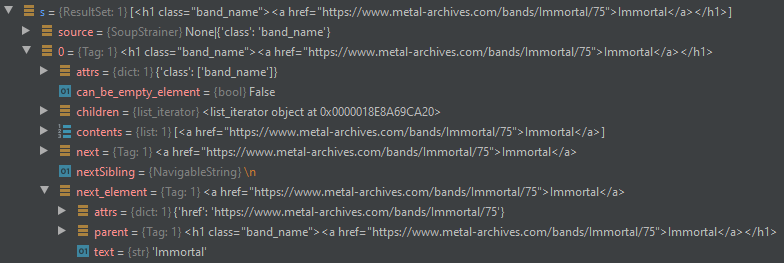
\includegraphics[scale=1.6]{debug_01}
      \end{center}
      
      % Don't ask.
      \texttt{band\_name} $=$ \texttt{s[0].next\_element.text}
    \end{frame}

  \subsection{Graph Databases}

    \begin{frame}{Comparison with a Relational Database}
    
      A relational database models connections between tables with foreign key relationships.
      
      \begin{center}
        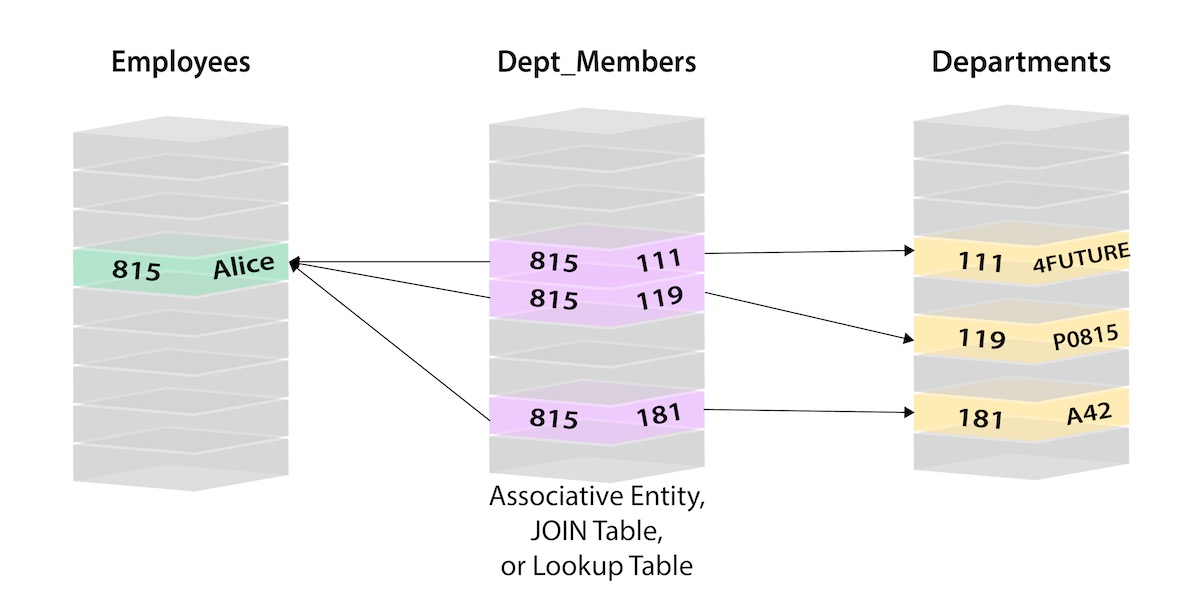
\includegraphics[scale=.2]{relational_as_graph}
      \end{center}
      
      https://neo4j.com/developer/graph-db-vs-rdbms/
      
    \end{frame}
    
    \begin{frame}{Modelling a Graph Database}

      A graph database consists of two elements: Nodes and edges.

      \begin{itemize}

        \item Nodes represent entities of data.
        \item Edges are the relationsips between nodes.\pause
        \item The former two are refined by properties (name/value pairs).
      \end{itemize}
      
      \begin{center}
        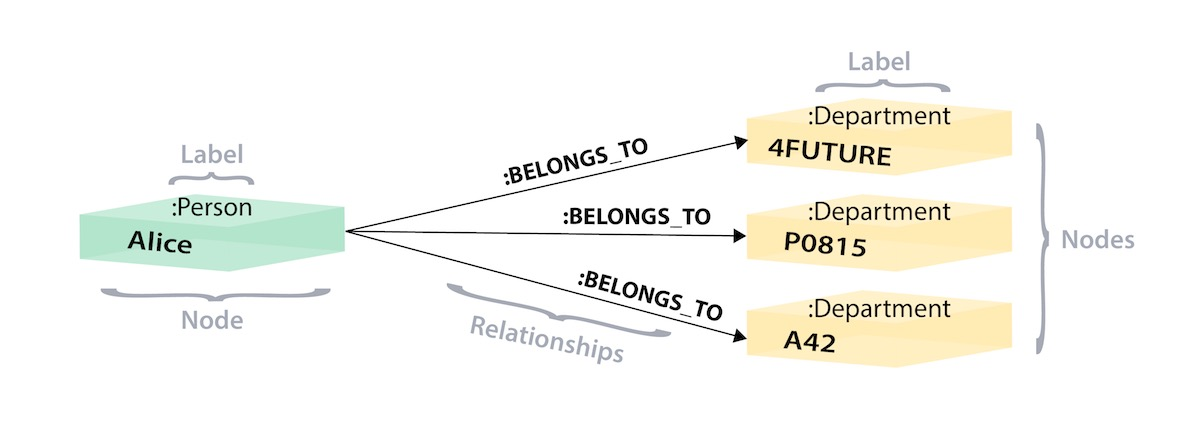
\includegraphics[scale=.2]{relational_graph_model}
      \end{center}
      
      Graphic: https://neo4j.com/developer/graph-database
      
    \end{frame}
    
    \begin{frame}{Modelling the Meta Metal Mapper database}
    
      Bands, Artists, Releases and Labels
    
    \end{frame}

  \subsection{Getting Serious}
  
    \begin{frame}{History - pt. 2}
    
    
    \end{frame}

%%%%%%%%%%%%%%%%%%%%%%%%%%%%%%%%%%%%%%%%%%%%%%%%%%%%%%%%%%%%%%%%%%%%%%%%%
%%%%%%%%%%%%%%%%%%%%%%%%%%%%%%%%%%%%%%%%%%%%%%%%%%%%%%%%%%%%%%%%%%%%%%%%%

\section{Exports and Reporting - Show, don't tell}

  \subsection{Band Networks}

    \begin{frame}{Scandinavia}
      Graphic
    \end{frame}

  \subsection{Country Statistics}

    \begin{frame}{Most Common Styles}
      Table?
    \end{frame}

\section{Résumé}

  \subsection{Statistics}

    \begin{frame}{Tools Used}
      \begin{itemize}
        \item<1-> Programming language: Python 2 and 3 on Window and Linux:
          \begin{itemize}
            \item<1-> certifi, urllib3, progressbar2, neomodel, beautifulsoup4, pyYAML

          \end{itemize}
        \item<1-> IDEs: Visual Studio and PyCharm,
        \item<1-> Neo4j (graph database)
        \item<1-> Graphviz (diagram rendering)
        \item<1-> SCM: git
        \item<1-> Gephi (graph rendering and querying)
        \item<1-> \LaTeX{}
        \item<1-> Markdown
      \end{itemize}
    \end{frame}
    
    \begin{frame}{Key Learnings}

      \begin{itemize}
        \item<1-> Know your tools, then learn some more.
        \item<1-> Don't be afraid to take risks.
        \item<2-> Don't be afraid of asking questions - Contacted \textit{HellBlazer}
      \end{itemize}

    \end{frame}
    
  \subsection{Link Collection}

    \begin{frame}{Further Reading}
      \begin{itemize}
        \item\href{https://musicmap.info/}{musicmap.info}: Musical genre development
          (not only metal) and influences over time.
        \item\href{https://www.boundbymetal.com/en/common/metal-genres-graph/}
          {boundbymetal.com}: Metal
          development from the beginning until 2010.
      \end{itemize}
    \end{frame}



\end{document}

    \begin{frame}{}

    \end{frame}


